\chapter{Pravidla hry Mastermind}

\subsubsection{Značení:}
V práci budeme používat následující značení:
\begin{itemize}
    \item Nechť $S$ je konečná množina. Potom $|S|$ značíme její mohutnost, tedy počet prvků.
    \item Formulí $\arg$ myslíme funkci, která vrátí prvek nabývající extrémní hodnoty popsané v navazujícím vzorci. Např $1 = \arg\max \{-x \mid x \in \mathbb{N}\}$.
    \item Nechť $K$ je množina. Symbolem $\mathcal{P}(K)$ značíme množinu všech podmnožin $K$.
\end{itemize}

Zavedeme definice potřebné pro vysvětlení průběhu hry Mastermind. Nejprve vymezíme prostor, se kterým pak dále budeme pracovat. 

\begin{definice}[Hammingův prostor]\label{def01:1}
  Nechť $n \in \N $, $k \in \N $. Potom množinu 
  \[ \{ u = u_1u_2 \dots u_n \hspace{2px} \mid \hspace{2px} u_i \in \{1, 2, 3, \dots, k\}, \hspace{2px} i \in \{1, 2, 3, \dots, n\} \}\]
  nazýváme n-dimenzionální k-ární Hammingův prostor a značíme ho $H_{n,k}$. Prvek $u \in H_{n,k}$ nazýváme kód.
\end{definice}
Číslo $n \in \N $ budeme nazývat počet pozic a $k \in \N $ počet barev. Číslu $u_i \in \{1, 2, 3, \dots, k\}$ budeme říkat barva. 


Pro nějaké dva kódy z $H_{n,k}$ zavedeme definici ohodnocení bílými a černými kolíčky inspirovanou D. Knuthem \cite{donald_e__knuth_1977} a D. Greenwellem \cite{greenwell}. 

Počet černých kolíčků pro nějaké dva kódy značí počet pozic, na kterých mají tyto kódy shodnou barvu. Formálně to zapíšeme v následující definici.

\begin{definice}[Počet černých kolíčků]\label{def01:2}
  Nechť $u,v \in H_{n,k}$ jsou kódy. Uvažujme množinu $\{i \in \{1,\dots, n\}\mid  u_i = v_i \}$. Počet černých kolíčků kódů $u$ a $v$ je velikost této množiny a značíme jej $b$. 
\end{definice}

% dříve: Pro $u$ a $v$ definujeme počet černých kolíčků jako $b = | \{i \in \{1,\dots, n\}\mid  u_i = v_i \}|$.  

Bílé kolíčky značí počet zbývajících pozic v prvním kódu, které se shodují s nějakou jinou pozicí v druhém kódu v barvě. Nejprve se vyhodnotí počet černých kolíčků a potom až počet bílých tak, aby každá pozice v obou kódech přispívala maximálně k jednomu kolíčku. Formálně to zapíšeme následující definicí. 

\begin{definice}[Počet bílých kolíčků]\label{defbilekol}
  Nechť $u,v \in H_{n,k}$ jsou kódy, $b$ je jejich počet černých kolíčků. 
  Označme $n_j$ počet výskytů barvy $j$ v kódu $u$, $m_j$ počet výskytů barvy $j$ v kódu $v$. 
  Potom počet bílých kolíčků kódů $u$ a $v$ dejinujeme jako 
  \[w = \sum_{j = 1}^k  \min(n_j, m_j) - b\]
\end{definice}

% přeformulovat jako poznámku???
Někdy nebudeme zdůrazňovat, že počet černých a bílých kolíčků patří k daným dvěma kódům, ale z kontextu to jasně plyne a budeme to předpokládat. 

\begin{definice}[Ohodnocení]\label{ohodnoceni}
  Nechť $u,v \in H_{n,k}$ jsou kódy, $b$ je počet černých kolíčků a $w$ je počet bílých kolíčků. 
  Ohodnocením kódů $u$ a $v$ myslíme uspořádanou dvojici $(b,w)$.
  Dále definujeme funkci $s \colon H_{n,k} \times H_{n,k} \to \mathbb{N}_0\times \mathbb{N}_0$, která dvojici kódů přiřadí jejich ohodnocení. Množinu všech ohodnocení v $H_{n,k}$ značíme $S$.
\end{definice}

Triviálním pozorováním je fakt, že součet černých a bílých kolíčků je maximálně n. To plyne z toho, že suma $\sum_{j = 1}^k  \min(n_j, m_j)$ z definice počtu bílých kolíčků je menší nebo rovna $n$. Zároveň v prostoru $H_{n,k}$ neexistuje ohodnocení $(n-1,1)$. Pokud se totiž kódy schodují právě na $n-1$ pozicích, musí se na poslední pozici lišit. 
\begin{tvrz}\label{pozmozneohodnoceni}
    Nechť $n \in \N$, $k \in \N, k>2$. Potom pro všechna $(b,w)\in \mathbb{N}_0 \times \mathbb{N}_0,\hspace{5px} b + w \leq n$ existuje dvojice kódů $u,v \in H_{n,k}$ taková, že jejich ohodnocení je $(b,w)$.
\end{tvrz}
\begin{dukaz}
    %Napřed dokážeme neexistenci ohodnocení $(n-1,1)$. Předpokládejme, že $n-1$ pozic je stejných v obou kódech $u$ a $v$. Předpokládejme dále, že se na poslední pozici $(i)$ liší. Nechť BÚNO nabývají na této pozici barvy $u_i = 1, v_i = 2$. Označme $k_l = |\{j\mid j \neq i, u_j = l\}|$ počet pozic s barvou $l$ v kódech $u$ a $v$ bez i-té pozice. Potom $n_j = m_j = k_j \hspace{5px} \forall j > 2, j \leq k$ ve značení definice \ref{defbilekol} a $n_1 = m_1 + 1 = k_1 + 1$, $m_2 = n_2 + 1 = k_2 + 1$. Tedy
    %\[w = \min(k_1 + 1, k_1) + \min(k_2, k_2 + 1) + \sum_{j = 3}^k  \min(k_j, k_j) - b = \sum_{j = 1}^k k_j - (n-1) = 0\]
    %díky rovnosti kódů na zbylých pozicích. Pokud se na poslední pozici shodují, jejich ohodnocení bude $(n,0)$. 

    Nyní dokážeme existenci ohodnocení pro $b+w \leq n$
    
    Nechť $w$ je sudé. Kódy zvolíme následovně:
\[
  u = 
    \underbrace{11\dots1}_{b}
    \underbrace{11\dots1}_{\frac{w}{2}}
    \underbrace{22\dots2}_{\frac{w}{2}}
    \underbrace{11\dots1}_{n-b-w}
 \]
 \[
  v = 
    \underbrace{11\dots1}_{b}
    \underbrace{22\dots2}_{\frac{w}{2}}
    \underbrace{11\dots1}_{\frac{w}{2}}
    \underbrace{22\dots2}_{n-b-w}
 \]
Vidíme, že počet černých kolíčků kódů $u$ a $v$ je $b$. Počet bílých kolíčků $w'$ je potom
\begin{align*} 
w' &= \min\left(n - \frac{w}{2}, b + \frac{w}{2}\right) + \min\left(\frac{w}{2}, n - b - \frac{w}{2}\right) - b \\ 
&= \min\left(n - b - \frac{w}{2}, \frac{w}{2}\right) + \min\left(\frac{w}{2}, n - b - \frac{w}{2}\right) \\
&= 2\cdot\min\left(\frac{w}{2}, n - b - \frac{w}{2}\right) = w
\end{align*}

V poslední rovnosti jsme využili předpokladu, že $b+w \leq n$, a tedy $\frac{w}{2} \leq n - b - \frac{w}{2}$

Pro $b+w \leq n$ a $w$ liché kódy zvolíme následovně:
\[
  u = 
    \underbrace{11\dots1}_{b}
    \underbrace{11\dots1}_{\frac{w-1}{2}}
    \underbrace{22\dots2}_{\frac{w-1}{2}-1}
    2
    3
    \underbrace{11\dots1}_{n-b-w}
 \]
 \[
  v = 
    \underbrace{11\dots1}_{b}
    \underbrace{22\dots2}_{\frac{w-1}{2}}
    \underbrace{11\dots1}_{\frac{w-1}{2}-1}
    3
    1
    \underbrace{22\dots2}_{n-b-w}
 \]
Počet černých kolíčků je $b$. Počet bílých kolíčků $w'$ kódů $u$ a $v$ je potom
\begin{align*} 
w' = \min\left(n-w+\frac{w-1}{2}, b + \frac{w-1}{2}\right) + \min\left(\frac{w-1}{2}, \frac{w-1}{2} + n-b-w\right) + \\ +\min(1,1) - b 
 = b + \frac{w-1}{2} + \frac{w-1}{2} + 1 - b = w
\end{align*}
\end{dukaz}

Silnější tvrzení platí pro případ se dvěma barvami. 

\begin{tvrz}\label{pozohodnoceniprodvebarvy}
    Nechť $n \in \N, k=2$. Nechť dále $u, v \in H_{n,k}$ jsou kódy s ohodnocením $(b,w)$. Potom $b + w \leq n, \hspace{5px} (b,w) \neq (n-1,1)$ a $w$ je sudé.
\end{tvrz}
\begin{dukaz}
$b + w \leq n, \hspace{5px} (b,w) \neq (n-1,1)$ platí obdobně jako v důkazu tvrzení \ref{pozmozneohodnoceni}. Kódy $u$ a $v$ lze permutací pozic dostat do následujícího tvaru
    \[
  u = 
    \underbrace{11\dots1}_{c}
    \underbrace{22\dots2}_{d}
    \underbrace{11\dots1}_{x}
    \underbrace{22\dots2}_{y}
 \]
 \[
  v = 
    \underbrace{11\dots1}_{c}
    \underbrace{22\dots2}_{d}
    \underbrace{22\dots2}_{x}
    \underbrace{11\dots1}_{y}
 \]
 kde $b = c + d$. 

 Potom
 \begin{align*}
     w &= \min(c + x, c + y) + \min(d + y, d + x) - b =\\
     &= \min(x, y) + \min(y, x) = 2\cdot \min(x, y)
 \end{align*}

\end{dukaz}

    
    %Nyní dokážeme, existenci ohodnocení pro nějaké $(b,w)$. Nechť napřed $w = 0$. Zvolme prvních $b$ pozic v obou kódech na barvu $1$. Protože $k>2$, můžeme pro zbylé pozice v prvním kódu zvolit barvu $1$ a pro zbylé pozice ve druhém kódu zvolit barvu $2$. Snadným ověřením z definice zjistíme, že tyto dva kódy mají ohodnocení $(b,0)$.   Nechť nyní $w > 0$ a $b+w < n$. První kód vytvoříme takto. Položme prvních $b$ pozic na barvu $1$. Položme dále dalších $w$ pozic v prvním kódu střídavě $1212\dots$ a zbylé pozice v prvním kódu vyplníme třetí barvou. Druhý kód vyplníme následovně. Položme prvních $b$ pozic na barvu $1$. Dalších $w + 1$ pozic zvolíme jako $212121\dots$ a kód doplníme barvou dva.     Pokud $b+w = n$ a $w$ je sudé. Náš postup bude fungovat s jedinou obměnou a to, že posledních posledních $w$ pozic druhého kódu $2121\dots$. Pokud $w$ je liché, zvolíme poseldních $w$ pozic prvního kódu $1212\dots3$ a posledních $w$ pozic druhého kódu $3121\dots$.





%V příkladu níže je ukázka konstrukce kódů s daným ohodnocením.
%\begin{prikl}
 %   Pro ohodnocení $(b,w), w > 0, b+w < n$ kódy mohou vypadat například takto:
  %  \[111111,1212121,33333\]
   % \[111111,21212121,2222\]

%    Pro případ $b+w = n$ a $w$ liché lze kódy sestavit takto:
 %   \[111111,1212123\]
  %  \[111111,3121212\]
%\end{prikl}

Nyní jsme připraveni definovat hru Mastermind. 

\section{Průběh hry Mastermind}
Nechť $n \in \N $, $k \in \N, m\in \N$. [n,k]-Mastermind je hra pro dva hráče 
% Šlo by oba hráče pojmenovat
% Cílem hry je nalézt tajný kód na co nejmenší počet pokusů. 
probíhající podle následujícího schématu. 
\begin{enumerate}
    \item První hráč vytvoří tajný kód $v \in H_{n,k}$.
    \item Hra dále probíhá po kolech $i = 1,2,\dots,m$:
        \begin{enumerate}
            \item Druhý hráč zadá kód (tah, pokus) $u_i \in H_{n,k}$.
            \item První hráč ohodnotí pokus s tajným kódem podle definice \ref{ohodnoceni}.
        \end{enumerate}
    \item Hra končí v případě, že pokus je ohodnocen $n$ černými kolíčky (zadaný kód se shoduje s tajným kódem), anebo je vyčerpán maximální počet pokusů m.
\end{enumerate}
Cílem hry [n,k]-Mastermind je nalézt tajný kód na co nejmenší počet pokusů. 

%\begin{definice}[\lbrack n,k\rbrack -Mastermind]\label{def01:2}
 %Nechť $n \in \mathbb{N}$, $k \in \mathbb{N}$. $v \in H_{n,k}$ je kód. Potom posloupnosti 
%\end{definice}

\begin{definice}[Ohodnocení v \lbrack n,k\rbrack -Mastermindu] \label{ohodnoceni2}
  Uvažujme [n,k]-Mastermind s tajným kódem $v \in H_{n,k}$.
  Ohodnocením kódu $u$ myslíme ohodnocení kódů $u$ a $v$.
\end{definice}

% přidat různé varianty hry mastermind??? např statická verze, hra pouze s kandidáty atd. 

V každém kole hry můžeme pojmenovat stav hry jako posloupnost pokusů s ohodnoceními. Stav přesně odpovídá informaci, kterou má hádající hráč k dispozici.
\begin{definice}[Stav]\label{stav}
   Uvažujme [n,k]-Mastermind s tajným kódem $v \in H_{n,k}$. 
   Nechť $u_i, i\in \{1,2,\dots m\}$ jsou kódy s ohodnoceními $r_i = (b_i,w_i) = s(u_i,v)$. Stav definujeme jako posloupnost $((u_1, r_1), \dots, (u_m, r_m))$.
\end{definice}










%%%%%%%%%%%%%%%%%%%%%%%%%%%% druha kapitola %%%%%%%%%%%%%%%%%%%%%%%%%%%%%%

\chapter{[4,6]-Mastermind}
Původní a nejrozšířenější variantou Mastermindu je použití čtyř pozic a šesti barev. 
% V úvodu popsat historii a základní variantu hry.
V následující kapitole popíšeme některé algoritmy, které [4,6]-Mastermind řeší a popíšeme jejich vlastnosti. Každý algoritmus skončí ve chvíli, kdy je pokus ohodnocen čtyřmi černými kolíčky. Díky tomu, že prostor kódů je konečný, tak algoritmus, který nezahraje žádný kód dvakrát, jistě skončí. Počet kol tedy nebudeme dále omezovat. 


Pro popis algoritmů řešící mastermind zavedeme pojem kandidát. Jde o kód, který má stejné ohodnocení s danou posloupností pokusů jako neznámý tajný kód. Podle dostupných informací by tedy kandidát mohl být tajným kódem.


\begin{definice}[kandidát]\label{kandidat}
  Uvažujme [n,k]-Mastermind s nějakým tajným kódem $v\in H_{n,k}$.
  Nechť $\left((u_1, r_1), (u_2,r_2), \dots, (u_j,r_j)\right), u_i \in H_{n,k}, r_i \in \N _0 \times \N _0$ je stav. Řekneme, že kód $u \in H_{n,k}$ je kandidát, pokud $s(u,u_i) = r_i \hspace{5px} \forall i \in \{1, \dots j\}$. 
  % Tohle není přesné - Pro prázdný stav řekneme, že každý kód $u \in H_{n,k}$ je kandidát. Množinu všech kandidátů budeme značit $K$.
\end{definice}


Definujeme tabulku rozdělení, která obsahuje mohutnosti množin kandidátů očíslované podle případných hodnocení dalšího pokusu. 

%\begin{definice}[Tabulka rozdělení]\label{tabrozdel}
  %Uvažujme [n,k]-Mastermind s nějakým tajným kódem $v\in H_{n,k}$.Nechť $\left((u_1, r_1), (u_2,r_2), \dots, (u_j,r_j)\right), u_i \in H_{n,k}, r_i \in \N _0 \times \N _0$ je stav. Uvažujeme nějaké seřazení všech možností ohodnocení $s_i \in \N_0\times\N_0, (s_1, s_2, \dots, s_m)$. Pro kód $u \in H_{n,k}$ definujeme tabulku rozdělení jako uspořádanou m-tici $(|K_1|, |K_1|, \dots, |K_m|)$, kde $K_i$ je množina kandidátů pro stav $\left((u_1,r_1), (u_2,r_2), \dots, (u_j,r_j), (u,s_i)\right)$.
%\end{definice}


% lemma, kdybychom pracovali se stavem i cestou
% místo lemmatu by šlo kandidáty definovat na grafu za pomoci cesty z vrcholu $H_{n,k}$
\begin{lemma}[Množina kandidátů a konec cesty]\label{kandidatacesta}
    Nechť $(V, E)$ je graf. Potom množina všech kandidátů stavu $\left((u_1, r_1), (u_2,r_2), \dots, (u_j,r_j)\right), u_i \in H_{n,k}, r_i \in \N _0 \times \N _0$ je rovna konci cesty $\left((u_1, r_1), (u_2,r_2), \dots, (u_j,r_j)\right), u_i \in H_{n,k}, r_i \in \N _0 \times \N _0$ z vrcholu $H_{n,k}$.
\end{lemma}
\begin{dukaz}
    Lemma dokážeme matematickou indukcí podle délky stavu (počtu kódů s ohodnocením). Nechť délka stavu je 1. Potom množina všech kandidátů stavu $(u_1, r_1)$ je množina $\{u \in H_{n,k} \mid s(u,u_1) = r_1\}$, což odpovídá definici potomku $H_{n,k}$ vzhledem ke kódu $u_1$ a ohodnocení $r_1$, který je koncem cesty $((u_1, r_1))$.

    Nechť lemma platí pro všechny stavy délky pro nějaké $l \in \N$. 
\end{dukaz}


%%%%%%%%%%%%%%%%%%%% poznámky %%%%%%%%%%%%%%%%%%%%%%%%%%%%
%Definujeme kořenový strom průběhu hry jako dvojici $(V, E)$, kde $V \subset \mathcal{P}(H_{n,k})$ je množina vrcholů, $E \subset \{(u_1, u_2) \mid (u_1, u_2) \in V \times V, u_1 \neq u_2\}$ je množina hran. 
  % \subset H_{n,k}

%Definujeme kořenový strom [n,k]-Mastermindu jako dvojici $(V, E)$. Každý vrchol $K$ má pouze potomky vzhledem k danému kódu $u$. $V \subset \mathcal{P}(H_{n,k})$ je množina složená z $H_{n,k}$. 

  % mozna bychom mohli pripustit i rovnost vrcholu v hrane, akorat by hrana vedla do stejneho vrcholu
  
  % kořenový strom musí být něco jiného než graf popisovaný výše. Musíme totiž ušetřit, že každý vrchol má pouze jednoho rodiče.

  
  
  %Řekneme, že hrana jsou všechny dvojice kód a nějaké ohodnocení $(u,r), u\in H_{n,k}, r \in S$. Jako kořen označíme množinu $H_{n,k}$. Pro vrchol $K \subset H_{n,k}$ definujeme jeho potomka vzhledem ke kódu $u\in H_{n,k}$ a ohodnocení $r \in S$ jako $K_{u,r} = \{w \in K \mid s(u,w) = r\}$. 
  %Nechť $\left((u_1, r_1), (u_2,r_2), \dots, (u_j,r_j)\right), u_i \in H_{n,k}, r_i \in \N _0 \times \N _0$ je stav. Řekneme, že kód $u \in H_{n,k}$ je kandidát, pokud $s(u,u_i) = r_i \hspace{5px} \forall i \in \{1, \dots j\}$. 
  % Tohle není přesné - Pro prázdný stav řekneme, že každý kód $u \in H_{n,k}$ je kandidát. Množinu všech kandidátů budeme značit $K$.


Definujeme tabulku rozdělení, která obsahuje mohutnosti množin kandidátů očíslované podle případných hodnocení dalšího pokusu. 

\begin{lemma}[Stav, cesta a kandidát]
    Množina všech kandidátů stavu $\left((u_1, r_1), (u_2,r_2), \dots, (u_j,r_j)\right), u_i \in H_{n,k}, r_i \in \N _0 \times \N _0$ je rovna vrcholu, na který se dostaneme z vrcholu $H_{n,k}$ cestou $\left((u_1, r_1), (u_2,r_2), \dots, (u_j,r_j)\right)$. 
    
\end{lemma}

\begin{lemma}[Množina kandidátů stavu a cesta v grafu]
    Množina všech kandidátů stavu $\left((u_1, r_1), (u_2,r_2), \dots, (u_j,r_j)\right), u_i \in H_{n,k}, r_i \in \N _0 \times \N _0$ je rovna vrcholu, 
    
\end{lemma}

\begin{definice}[Tabulka rozdělení]\label{tabrozdel}
  Uvažujme [n,k]-Mastermind s nějakým tajným kódem $v\in H_{n,k}$.
  Nechť $\left((u_1, r_1), (u_2,r_2), \dots, (u_j,r_j)\right), u_i \in H_{n,k}, r_i \in \N _0 \times \N _0$ je stav. 
  Uvažujeme množinu všech možných ohodnocení v $H_{n,k}. $\[S = \{s_1, s_2, \dots, s_m\}, s_i \in \N_0\times\N_0\]
  
  Dále označíme $S$ množinu všech možností ohodnocení $s_i \in \N_0\times\N_0, S = \{s_1, s_2, \dots, s_m\}$. 
  %Uvažujeme nějaké seřazení všech možností ohodnocení $s_i \in \N_0\times\N_0, (s_1, s_2, \dots, s_m)$. 
  Pro kód $u \in H_{n,k}$ definujeme tabulku rozdělení jako uspořádanou m-tici $(|K_1|, |K_1|, \dots, |K_m|)$, kde $K_i$ je množina kandidátů pro stav $\left((u_1,r_1), (u_2,r_2), \dots, (u_j,r_j), (u,s_i)\right)$.
\end{definice}

\begin{definice}[Neprázdný stav]
    Uvažujeme [n,k]-Mastermind s nějakým tajným kódem $v\in H_{n,k}$. Řekneme, že stav $\left((u_1, r_1), (u_2,r_2), \dots, (u_j,r_j)\right), u_i \in H_{n,k}, r_i \in \N _0 \times \N _0$ je neprázdný, pokud je množina všech kandidátů tohoto stavu neprázdná. 
\end{definice}

\begin{definice}[Rozdělení]
    Uvažujeme [n,k]-Mastermind s nějakým tajným kódem $v\in H_{n,k}$. Pro neprázdný stav $\left((u_1, r_1), (u_2,r_2), \dots, (u_j,r_j)\right), u_i \in H_{n,k}, r_i \in \N _0 \times \N _0$ a kód $u \in H_{n,k}$ definujeme rozdělení jako množinu stavů $\left((u_1, r_1), (u_2,r_2), \dots, (u_j,r_j), (u, r)\right), u_i \in H_{n,k}, r_i \in \N _0 \times \N _0$. , pokud je množina všech kandidátů tohoto stavu neprázdná. 
\end{definice}

Tabulku rozdělení si lze představit jako pravděpodobnostní rozdělení, kde pravděpodobnost ohodnocení $s_i$ je $\frac{|K_i|}{|K|}$. Z teorie grafů můžeme tabulku rozdělení využít pro vytvoření kořenového stromu, kde vrchol je množina kandidátů $K$. Jeho děti pak jsou $K_1, K_1, \dots, K_m$ ve smyslu právě zmíněné definice pro nějaký kód $u$. Daný strom pak může korespondovat s průběhem hry Mastermind, kdy každá vrstva odpovídá jednomu kolu. Stav hry v tomto smyslu vyjádříme jako množinu kandidátů. 


%%%%%%%%%%%%%%%%%%%%%%%%%%%%%% příklad [2,3]-Mastermind %%%%%%%%%%%%%
\subsubsection{příklad}
\begin{prikl}\label{malyprikladminmax}
    V tabulce \ref{tabmalyminmaxprvnitah} jsou maximální hodnoty tabulek rozdělení pro dva první tahy $11$, $12$. Vidíme, že jsou obě hodnoty shodné. Knuthův algoritmus tedy vybere jako první tah kód 11, protože je první v lexikografickém pořadí a oba kódy jsou kandidáti. 


\begin{table}[h]
\centering
\begin{tabular}{l l l}
\toprule
kód & 11 & 12  \\
\midrule
maximum & 4 & 4\\
\bottomrule
\end{tabular}
\caption{Maximum tabulek rozdělení pro první tah}\label{tabmalyminmaxprvnitah}
\end{table}


Kód $11$ může dostat celkem tři ohodnocení, $(0,0), (1,0), (2,0)$. Ohodnocení $(0,1), (0,2)$ nemůže dostat, protože pokud tajný kód obsahuje barvu $1$, potom v ohodnocení nutně bude nějaký černý kolíček. Pokud je ohodnocení $(2,0)$, hra končí. Pro další dvě možné ohodnocení uvádíme v tabulce \ref{tabdruhytahmalyminmax} maximální hodnoty tabulek rozdělení pro všechny kódy. Tučně jsou zobrazeny hodnoty u kandidátů.


\begin{table}[h]
\centering
\begin{tabular}{l l l l l l l l l l}
\toprule
kód & 11 & 12 & 13 & 21 & 22 & 23 & 31 & 32 & 33\\
\midrule
(0,0) & 4& 2& 2& 2& \textbf{2}& \textbf{2}& 2& \textbf{2}& \textbf{2}\\
(1,0) & 4& \textbf{1}& \textbf{1}& \textbf{1}& 2& 2& \textbf{1}& 2& 2\\
\bottomrule
\end{tabular}
\caption{Maximum tabulek rozdělení pro druhý tah v závislosti na ohodnocení prvního pokusu}\label{tabdruhytahmalyminmax}
\end{table}


Jako druhý tah tedy Knuthův algoritmus zvolí kód $22$ v případě ohodnocení prvního tahu $(0,0)$ a kód $12$ v případě ohodnocení prvního tahu $(1,0)$. 

Nyní vybereme třetí tah. Zajímavá je pouze situace v případě druhého tahu $22$. Tabulka \ref{tabmalyminmaxtabrozdeldruhytah} ukazuje tabulku rozdělení pro tento kód a stav $(((1,1),(0,0)))$. 

\begin{table}[h]
\centering
\begin{tabular}{l l l l l l}
\toprule
ohodnocení & (0,0) & (0,1) & (0,2) & (1,0) & (2,0)\\
\midrule
počet kandidátů & 1& 2& 0& 0& 1\\
\bottomrule
\end{tabular}
\caption{Tabulka rozdělení pro druhý tah 22}\label{tabmalyminmaxtabrozdeldruhytah}
\end{table}

Tabulka \ref{tabmalyminmaxtretitahtabrozdel} uvádí maximální hodnoty tabulek rozdělení pro stav $(((1,1),(0,0)), ((2,2),(0,1)))$ a jednotlivé kódy. Tučně uvedené jsou opět hodnoty pro kandidáty. Knuthův algoritmus tedy v tomto případě jako třetí tah zvolí kód $23$. 

\begin{table}[h]
\centering
\begin{tabular}{l l l l l l l l l l}
\toprule
kód & 11 & 12 & 13 & 21 & 22 & 23 & 31 & 32 & 33\\
\midrule
maximum tabulky rozdělení & 2& 1& 1& 1& 2& \textbf{1}& 1& \textbf{1}& 2\\
\bottomrule
\end{tabular}
\caption{Maximum tabulek rozdělení pro třetí tah}\label{tabmalyminmaxtretitahtabrozdel}
\end{table}

Volby pokusů jsou přehledněji znázorněny na obrázku \ref{fig23start11}. Vrcholy značí zvolené pokusy a hrany možná ohodnocení.


\begin{figure}[h]
    \centering
    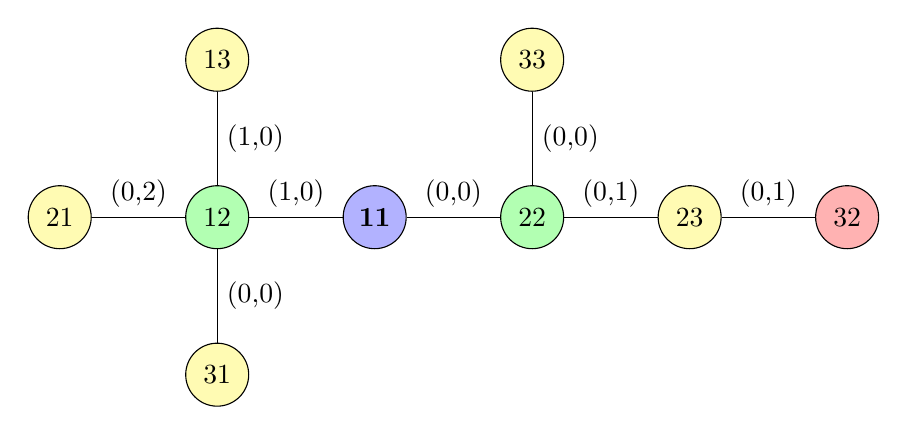
\begin{tikzpicture}
    \node[draw, circle, fill=blue!30, minimum size=8mm] (1) at (0,0) {\textbf{11}};
    \node[draw, circle, fill=green!30, minimum size=8mm] (2) at (2,0) {22};
    \draw (1) -- (2) node[pos=0.5, above] {(0,0)};
        \node[draw, circle, fill=yellow!30, minimum size=8mm] (3) at (2,2) {33};
        \draw (2) -- (3) node[pos=0.5, right] {(0,0)};
        \node[draw, circle, fill=yellow!30, minimum size=8mm] (4) at (4,0) {23};
        \draw (2) -- (4) node[pos=0.5, above] {(0,1)};
        \node[draw, circle, fill=red!30, minimum size=8mm] (5) at (6,0) {32};
        \draw (4) -- (5) node[pos=0.5, above] {(0,1)};
    \node[draw, circle, fill=green!30, minimum size=8mm] (6) at (-2,0) {12};
    \draw (1) -- (6) node[pos=0.5, above] {(1,0)};
    \node[draw, circle, fill=yellow!30, minimum size=8mm] (7) at (-2,-2) {31};
    \draw (6) -- (7) node[pos=0.5, right] {(0,0)};
    \node[draw, circle, fill=yellow!30, minimum size=8mm] (8) at (-4,0) {21};
    \draw (6) -- (8) node[pos=0.5, above] {(0,2)};
    \node[draw, circle, fill=yellow!30, minimum size=8mm] (9) at (-2,2) {13};
    \draw (6) -- (9) node[pos=0.5, right] {(1,0)};
    \end{tikzpicture}
    \caption{Zahrané tahy podle ohodnocení}
    \label{fig23start11}
\end{figure}

    Algoritmus min-max vyhraje [2,3]-Mastermind na maximálně čtyři pokusy. Lze hru vyhrát na menší počet pokusů? Obrázek \ref{fig23start12} ukazuje zahrané tahy Knuthovým algoritmem v případě prvního pokusu $12$. Pozorujeme, že v tomto případě stačí maximálně tři pokusy na nalezení tajného kódu. 

    
\begin{figure}[h!]
    \centering
    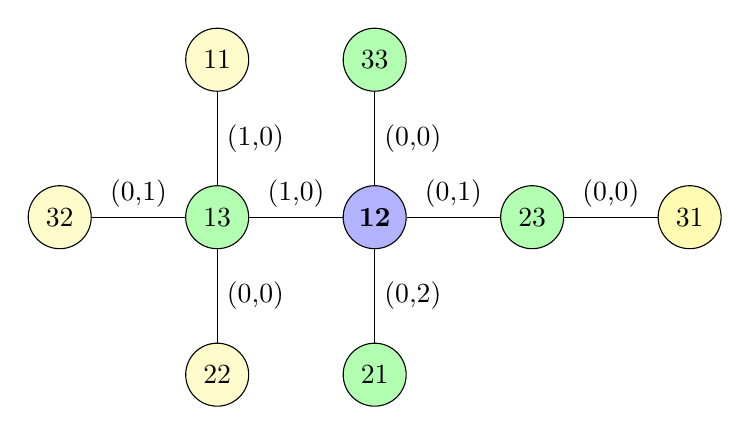
\begin{tikzpicture}
    \node[draw, circle, fill=blue!30, minimum size=8mm] (1) at (0,0) {\textbf{12}};
    \node[draw, circle, fill=green!30, minimum size=8mm] (2) at (0,2) {33};
    \draw (1) -- (2) node[pos=0.5, right] {(0,0)};
    \node[draw, circle, fill=green!30, minimum size=8mm] (3) at (2,0) {23};
    \draw (1) -- (3) node[pos=0.5, above] {(0,1)};
    \node[draw, circle, fill=yellow!30, minimum size=8mm] (4) at (4,0) {31};
    \draw (3) -- (4) node[pos=0.5, above] {(0,0)};
    \node[draw, circle, fill=green!30, minimum size=8mm] (5) at (0,-2) {21};
    \draw (1) -- (5) node[pos=0.5, right] {(0,2)};
    \node[draw, circle, fill=green!30, minimum size=8mm] (6) at (-2,0) {13};
    \draw (1) -- (6) node[pos=0.5, above] {(1,0)};
    \node[draw, circle, fill=yellow!20, minimum size=8mm] (7) at (-2,-2) {22};
    \draw (6) -- (7) node[pos=0.5, right] {(0,0)};
    \node[draw, circle, fill=yellow!20, minimum size=8mm] (8) at (-4,0) {32};
    \draw (6) -- (8) node[pos=0.5, above] {(0,1)};
    \node[draw, circle, fill=yellow!20, minimum size=8mm] (9) at (-2,2) {11};
    \draw (6) -- (9) node[pos=0.5, right] {(1,0)};
    \end{tikzpicture}
    \caption{Zahrané tahy podle ohodnocení}
    \label{fig23start12}
    \end{figure}

\end{prikl}

Tento příklad ilustruje omezení min-max algoritmu. Může se totiž stát, že výsledný počet tahů je lepší v případě zvolení jiného počátečního tahu. Výsledky budou dále diskutovány v kapitole $3$.


Prvním algoritmem je metoda, kterou navrhl D. Knuth \cite{donald_e__knuth_1977}. Odpovídá algoritmu \ref{jednokrokalgorithm} se vstupní jednokrokovou funkcí $m_K$ a funkcionálem $M$.

Jeho algoritmus vybírá pro další pokus ten kód, který minimalizuje maximální hodnotu v tabulce rozdělení. 

Formálně tento postup můžeme zapsat následovně. Nechť $v\in H_{4,6}$ a \hfill \break $\left((u_1, r_1), (u_2,r_2), \dots, (u_j,r_j)\right), u_i \in H_{n,k}, r_i \in \N _0 \times \N _0$ je stav. Pro $w \in H_{4,6}$ označme $K^w$ příslušnou tabulku rozdělení. Potom Knuthův algoritmus vybere jako další pokus vektor, který je řešením následujícího problému minimalizace.

\[ u = \arg\min_{w \in H_{4,6}} \max_{|K^u_i|} \{ |K^u_i| \in K^u\} \]

Formulí $\arg$ myslíme funkci, která vrátí prvek nabývající extrémní hodnoty popsané v navazujícím vzorci. V případě nejednoznačného řešení min max problému preferuje Knuthův algoritmus výběr kandidátů a dále lexikografické pořadí. Těmito kritérii docílíme vždy jednoznačného výběru dalšího pokusu. 

\begin{prikl}\label{prminmaxprvnipokus}
    Tabulka \ref{tab02} ukazuje v řádku maximální hodnoty tabulek rozdělení pro první tahy. Knuthův algoritmus tedy jako první tah používá kód $1122$. 
\end{prikl}

Následující příklad ukazuje vybrané pokusy v [2,2]-Mastermindu zvolené Knuthovým algoritmem. Zároveň tento příklad poukazuje na možné nedostatky popisovaného algoritmu. Výsledky jsou podrobněji popsány ve třetí kapitole.

Chod Knuthova algoritmu nastíníme na [2,2]-Mastermindu. 
\subsubsection{[2,2]-Mastermind}
Prostor kódů [2,2]-Mastermindu je množina $H_{2,2} = \{11,12,21,22\}$. Množina všech ohodnocení je podle tvrzení \ref{tvrzohodnoceni2} rovna $S = \{(0,0), (0,2), (1,0), (2,0)\}$. Na obrázku \ref{fig22prvnitah11} a \ref{fig22prvnitah12} jsou zobrazeny potomci $H_{2,2}$ vzhledem ke kódu $11$ a $12$. Případy s kódy $22$ a $21$ jsou obdobné zmíněným kódům díky rovnoměrnému rozdělení kódů. Protože kódy $22$ a $21$ jsou lexikograficky vyšší, nemusíme je rozebírat. 
\begin{figure}[h!]
    \centering
    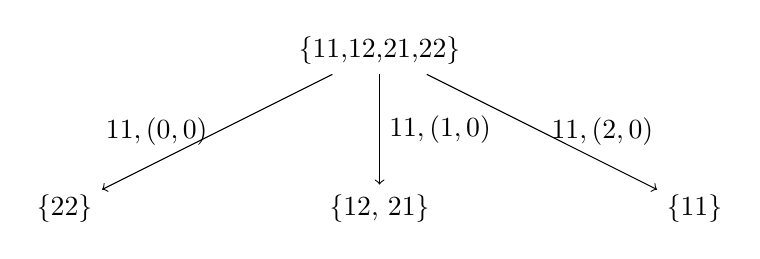
\begin{tikzpicture}
    \node (1) at (0,0) {\{11,12,21,22\}};
    
    \node (2) at (-4,-2) {\{22\}};
    \draw[->] (1) -- (2) node[pos=0.5, left] {$11,(0,0)$};
    \node (3) at (0,-2) {\{12, 21\}};
    \draw[->] (1) -- (3) node[pos=0.5, right] {$11,(1,0)$};
    \node (5) at (4,-2) {\{11\}};
    \draw[->] (1) -- (5) node[pos=0.5, right] {$11,(2,0)$};

    \end{tikzpicture}
    \caption{První tah, obdobný s grafem pro 22}
    \label{fig22prvnitah11}
    \end{figure}
\begin{figure}[h!]
    \centering
    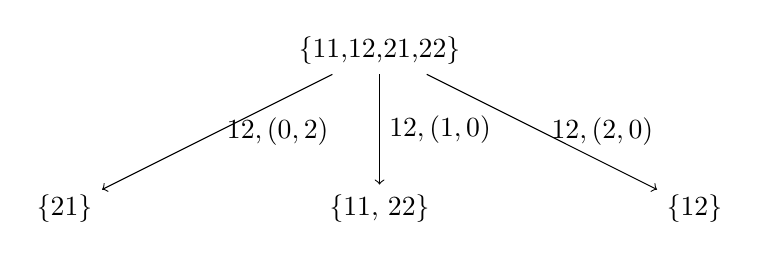
\begin{tikzpicture}
    \node (1) at (0,0) {\{11,12,21,22\}};
    
    \node (4) at (-4,-2) {\{21\}};
    \draw[->] (1) -- (4) node[pos=0.5, right] {$12,(0,2)$};
    \node (5) at (0,-2) {\{11, 22\}};
    \draw[->] (1) -- (5) node[pos=0.5, right] {$12,(1,0)$};
    \node (6) at (4,-2) {\{12\}};
    \draw[->] (1) -- (6) node[pos=0.5, right] {$12,(2,0)$};

    \end{tikzpicture}
    \caption{První tah, obdobný s grafem pro 21}
    \label{fig22prvnitah12}
\end{figure}

Hodnoty $m_{H_{2,2}}$ jsou tedy následující. 
\[m_{H_{2,2}} (11) = m_{H_{2,2}} (12) = m_{H_{2,2}} (21) = m_{H_{2,2}} (22) = 2\]
Knuthův algoritmus volí jako první pokus kód $11$. 
\begin{figure}[h!]
    \centering
    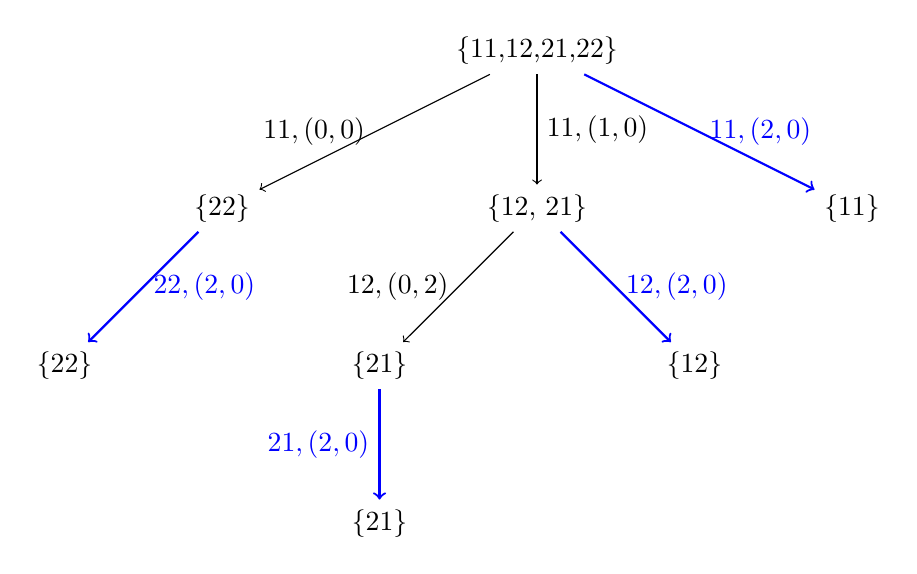
\begin{tikzpicture}
    \node (1) at (0,0) {\{11,12,21,22\}};
    \node (2) at (-4,-2) {\{22\}};
    \draw[->] (1) -- (2) node[pos=0.5, left] {$11,(0,0)$};
    \node (3) at (0,-2) {\{12, 21\}};
    \draw[->] (1) -- (3) node[pos=0.5, right] {$11,(1,0)$};
    \node (4) at (4,-2) {\{11\}};
    \draw[->, thick, blue] (1) -- (4) node[pos=0.5, right] {$11,(2,0)$};
    \node (5) at (-2,-4) {\{21\}};
    \draw[->] (3) -- (5) node[pos=0.5, left] {$12,(0,2)$};
    \node (6) at (2,-4) {\{12\}};
    \draw[->, thick, blue] (3) -- (6) node[pos=0.5, right] {$12,(2,0)$};
    \node (7) at (-6,-4) {\{22\}};
    \draw[->, thick, blue] (2) -- (7) node[pos=0.5, right] {$22,(2,0)$};
    \node (8) at (-2,-6) {\{21\}};
    \draw[->, thick, blue] (5) -- (8) node[pos=0.5, left] {$21,(2,0)$};
    \end{tikzpicture}
    \caption{První a druhý tah}
\label{fig22dvatahy}
\end{figure}

Na obrázku \ref{fig22dvatahy} jsou doplněny potomci všech vrcholů až do dosažení ohodnocení $(2,0)$, kdy hra končí. Platí, že $m_K(u) \geq 1$ pro $K \neq \emptyset$. Proto, když lexikograficky nejnižší kandidát $u$ dosahuje hodnoty $m_K(u) = 1$, algoritmus min-max ho vždy vybere. Ukazuje se, že to je případ pro všechny zbývající vrcholy, $\{22\}, \{12, 21\}, \{21\}$.
    
\begin{figure}[h!]
    \centering
    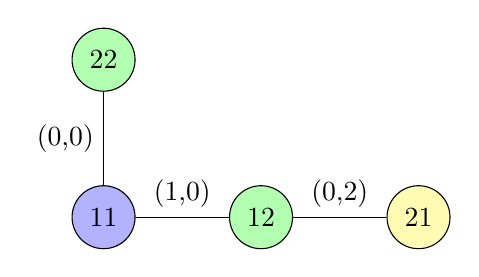
\begin{tikzpicture}
    \node[draw, circle, fill=blue!30, minimum size=8mm] (1) at (0,0) {11};
    \node[draw, circle, fill=green!30, minimum size=8mm] (2) at (0,2) {22};
    \draw (1) -- (2) node[pos=0.5, left] {(0,0)};
    \node[draw, circle, fill=green!30, minimum size=8mm] (3) at (2,0) {12};
    \draw (1) -- (3) node[pos=0.5, above] {(1,0)};
    \node[draw, circle, fill=yellow!30, minimum size=8mm] (4) at (4,0) {21};
    \draw (3) -- (4) node[pos=0.5, above] {(0,2)};
    
    \end{tikzpicture}
    \caption{Zahrané tahy podle ohodnocení}
    \label{fig23start12}
\end{figure}




% Přidat pseudokód algoritmu???

%vysledky Knuthova algoritmu:
% zdroj - Kooi
%expected - 4.476
% maximal - 5
% použít svůj kód a ocitovat

\subsection{entropie}
Neuwirth \cite{neuwirth} 
% Asi Neuwirth, chtělo by ale najít článek Irwinga.
navrhl algoritmus hrající tahy, které maximalizují entropii tabulky rozdělení. Nejprve však musíme definovat, co si vlastně pod entropií tabulky rozdělení můžeme představit a jaký má pro nás entropie význam.

\begin{definice}[Entropie]\label{defentropie}
  Nechť $A$ je konečná množina, $P \colon A \to [0,1]$ je zobrazení takové, že $\sum_{a \in A} P(a) = 1$. Nechť $s(P) = \{ a \in A \mid P(a) > 0\}$. Potom entropii zobrazení $P$ definujeme jako 
  \[H(P) = \sum_{a \in s(P)}P(a)\log_2\left(\frac{1}{P(a)}\right)\]
  Zobrazení $P$ budeme říkat rozdělení, dané hodnotě $P(a)$ pravděpodobnost a množině $[0,1]$ pravděpodobnostní prostor. 
\end{definice}

\begin{definice}[Entropie tabulky rozdělení]\label{defentropietabrozdel}
  Uvažujme [n,k]-Mastermind s tajným kódem $v$. Nechť $K$ množina kandidátů, $u \in H_{n,k}$ a $K^u = (|K^u_1|, |K^u_1|, \dots, |K^u_m|)$ je jeho tabulka rozdělení. Potom entropii tabulky rozdělení definujeme jako
  \[H(K^u) = \sum_{i=1}^n \frac{|K^u_i|}{|K|}\log_2\left( \frac{|K|}{|K^u_i|} \right)\]
\end{definice}

\begin{pozn}
    Definice \ref{defentropietabrozdel} koresponduje s definicí entropie pro množinu všech ohodnocení $A = \{s_1, s_2, \dots, s_m \}$ a zobrazení $P\colon A \to [0,1], P(s_i) = \frac{|K^u_i|}{|K|}$.
\end{pozn}

Co nám ale tato definice říká? Intuici za definicí entropie nastíníme v příkladu \ref{prbinarysearch}, který dává určitou smysl pro výraz $\log_2\left(\frac{1}{P(a)}\right)$ a příkladu \ref{prentropierozdeleni}, který ukazuje příklad entropie na konkrétním rozdělení.

Představme si, že chceme uhodnout tajné číslo z množiny $\{1,2,\dots,8\}$ pokládáním nějakých ano/ne otázek. Předpokládejme, že každé číslo může být tajným číslem se stejnou pravděpodobností $\frac{1}{8}$. Známým postupem, jak tajné číslo najít je takzvaným půlením intervalu (binární vyhledávání). Vždy se zeptáme, zda je číslo větší nebo menší než číslo v polovině. Tento postup je znázorněn v příkladu \ref{prbinarysearch}.

\begin{prikl}[Binární vyhledávání]\label{prbinarysearch}
Nechť tajné číslo je 4. Binární vyhledávání by mělo následující průběh:

Otázka: "Je číslo větší než 4?". 
Odpověď: ne

Otázka: "Je číslo větší než 2?". 
Odpověď: ano

Otázka: "Je číslo větší než 3?". 
Odpověď: ano

Výsledné číslo je 4. Počet otázek nutných k určení tajného čísla je 3.
\end{prikl}

\begin{pozn}\label{poznotazkynamnozinu}
Obdobně jako v příkladu \ref{prbinarysearch} lze pro jakoukoliv osmiprvkovou množinu $A$ s rovnoměrnou pravděpodobností vytvořit sadu otázek ano/ne a o každém prvku této množiny určit, zda odpovídá odpovědi ano nebo odpovědi ne. Následně bychom mohli pro určení jakéhokoliv prvku této množiny aplikovat obdobný postup jako v příkladu \ref{prbinarysearch}. Pro vhodnou sadu otázek existuje postup, který každou otázkou rozdělí prostor zbývajících možností na polovinu. Tím pádem pro určení jakéhokoliv prvku množiny $A$ potřebujeme $\log_2(|A|)$ otázek. 
\end{pozn}

\begin{prikl}\label{prentropierozdeleni}
Nechť $A = \{ \text{a, b, c, d}\}$ a $P$ je zadaná následovně: 
\[P(a) = \frac{1}{8}, P(b) = \frac{1}{8}, P(c) = \frac{1}{4}, P(d) = \frac{1}{2}\]
Nyní si představme pravděpodobnostní prostor jako čtverec na obrázku \ref{prprostor}, kde pravděpodobnost prvku je velikost plochy. Výraz $\frac{1}{P(a)}$ říká, kolik prvků $A$ s touto pravděpodobností by se "vešlo" do pravděpodobnostního prostoru jako na obrázku. Například dílek c by se "vešel" do pravděpodobnostního prostoru čtyřikrát.
Hodnota $\log_2\left(\frac{1}{P(c)}\right)$ lze interpretovat jako počet otázek ano/ne, který potřebujeme k jednoznačnému určení prvku c v případě, kdyby byl pravděpodobnostní prostor rozdělen rovnoměrně. Tento postup byl popsán v příkladu \ref{prbinarysearch} a v diskuzi pod ním.
Entropie tohoto rozdělení by v tomto případě byla 
\[H(P) = \frac{1}{8}\log_2 (8) + \frac{1}{8}\log_2 (8) + \frac{1}{4}\log_2 (4) + \frac{1}{2}\log_2 (2) = \frac{3}{8} + \frac{3}{8} + \frac{2}{4} + \frac{1}{2} = \frac{7}{4}\]
a můžeme ji interpretovat jako vážený průměr počtu otázek, který potřebujeme k jednoznačnému určení prvku z množiny $A$. 


\begin{figure}
\begin{tikzpicture}
    \draw[black, thick] (0,0) rectangle (4,4);
    \begin{scope}
        \node (1) at (1,0.5) {a - 1/8}
        \node (2) at (1,1.5) {b - 1/8}
        \node (3) at (1,3) {c - 1/4}
        \node (4) at (3,2) {d - 1/2}
    \end{scope}
    \draw[black, thick] (2,0) -- (2,4);
    \draw[black, thick] (0,2) -- (2,2);
    \draw[black, thick] (0,1) -- (2,1);

    
\end{tikzpicture}
\caption{Pravděpodobnostní prostor}
\label{prprostor}
\end{figure}

\end{prikl}

Nyní jsme připraveni na to, abychom vysvětlili, jakým způsobem aplikujeme výpočet entropie na strategii pro řešení [4,6]-Mastermindu.

Nechť $K$ je aktuální množina kandidátů, $u \in H_{4,6}$ je kód a $(|K_1|, |K_2|,\dots, |K_m|)$ je tabulka rozdělení pro kód $u$. Pro každé $K_i, i \in \{1, 2, \dots, m\}$ můžeme ve smyslu poznámky \ref{poznotazkynamnozinu} definovat nějakou abstraktní hodnotu počtu otázek ano/ne potřebných k určení jakéhokoliv prvku  $x \in K_i$ jako $\log_2(|K_i|)$. Potom obdobně jako v příkladu \ref{prentropierozdeleni} můžeme určit očekávaný počet otázek jako
\[G = \sum_{i =1}^n \frac{|K_i|}{|K|}\log_2|K_i| \]
Tato hodnota bude naším stavebním kamenem pro strategii za užití entropie. Protože cílem [4,6]-Mastermindu je najít tajný kód v co nejmenším počtu pokusů, chceme hodnotu $G$ minimalizovat. 

\[ u = \arg\min_{w \in H_{4,6}} \sum_{i =1}^n \frac{|K_i|}{|K|}\log_2|K_i|\]

\begin{lemma}[Aritmetika min a max]
    Nechť $K$ je konečná množina a $f \colon K \to \mathbb{R}$ je funkce. Nechť $a \in \mathbb{R}, a > 0$. Potom 
    \[f(x) = \min_{z \in K} f(z)\]
    právě tehdy když
    \[a\cdot f(x) = \min_{z \in K} a\cdot f(z)\]
    Obdobné tvrzení platí pro $\max$.
\end{lemma}
\begin{dukaz}
    $f(x) = \min_{z \in K} f(z)$ právě tehdy, když $\forall z \in K\colon \hspace{5px} f(x) \leq f(z)$. To platí právě tehdy, když $\forall z \in K\colon \hspace{5px} a \cdot f(x) \leq a\cdot f(z)$, což je ekvivalentní tvrzení \[a\cdot f(x) = \min_{z \in K} a\cdot f(z)\]
\end{dukaz}


\begin{tvrz}[Aritmetika min a max]
    Nechť $K$ je konečná množina a $f \colon K \to \mathbb{R}$ je funkce. Nechť $a \in \mathbb{R}, a < 0$. Potom 
    \[f(x) = \min_{z \in K} f(z)\]
    právě tehdy když
    \[a\cdot f(x) = \max_{z \in K} a\cdot f(z)\]
    Tvrzení platí i při záměnně $\min$ a $\max$.
\end{tvrz}
\begin{dukaz}
    $f(x) = \min_{z \in K} f(z)$ právě tehdy, když $\forall z \in K\colon \hspace{5px} f(x) \leq f(z)$. To platí právě tehdy, když $\forall z \in K\colon \hspace{5px} a \cdot f(x) \geq a\cdot f(z)$, protože $a<0$. To je ekvivalentní tvrzení \[a\cdot f(x) = \max_{z \in K} a\cdot f(z)\]
\end{dukaz}


\begin{veta}[Logaritmus a střední hodnota]
    \[\sum_{i=1}^{n} \frac{|K^u_i|}{|K|} \log_2|K^u_i| = \min_{w \in H_{4,6}} \sum_{i=1}^n \frac{|K^w_i|}{|K|}\log_2|K^w_i|\] 
    právě tehdy když
    \[\sum_{i=1}^{n} \frac{|K^u_i|}{|K|} \log_m|K^u_i| = \min_{w \in H_{4,6}} \sum_{i=1}^n \frac{|K^w_i|}{|K|}\log_m|K^w_i|\] 
\end{veta}
\begin{dukaz}
    Platí, že 
    \[\log_y x = \frac{\log x}{\log y}\]
    \[\log_z x = \frac{\log x}{\log z}\]
    tedy
    \[\log_y x = \log_z x \cdot \frac{\log z}{\log y}\]
    Navíc 
    \[\frac{\log z}{\log y}\]
    je konstantní v závislosti na $x$.
    Obdobně
    \[\frac{\log2}{\log m} \cdot\sum_{i=1}^{n} \frac{|K^u_i|}{|K|} \log_2|K^u_i| 
    = \frac{\log2}{\log m} \cdot \min_{w \in H_{4,6}} \sum_{i=1}^n \frac{|K^w_i|}{|K|}\log_2|K^w_i|
    = \min_{w \in H_{4,6}} \sum_{i=1}^n \frac{|K^w_i|}{|K|}\log_m|K^w_i| \]
    Protože $m > 1$, tak platí, že $\frac{\log2}{\log m} > 0$ a tedy lze využít vlastnosti minima a vnořit konstantu dovnitř výrazu. 
    % zde by možná chtělo citovat nějaká skripta s aritmetikou ohledně min a max tvarů.
\end{dukaz}

% Přidat definici entropie tabulky rozdělení.
\begin{veta}[Ekvivalence maximalizace entropie] \label{ekvivalencemaxentropy}
    Uvažujme [4,6]-Mastermind s tajným kódem $v\in H_{4,6}$ a máme posloupnost pokusů $\left(u_1, u_2, \dots, u_j\right), u_i \in H_{4,6}$ s ohodnoceními $\lbrack (b_1,w_1) , (b_2,w_2), \dots, (b_j,w_j)\rbrack)$. Označme $K$ množinu kandidátů pro tuto posloupnost pokusů. Pro $w \in H_{4,6}$ označme $K^w$ příslušnou tabulku rozdělení. Potom 
    \[u = \arg\min_{w \in H_{4,6}} \sum_{i=1}^n \frac{|K^w_i|}{|K|}\log_2|K^w_i|\]
    právě tehdy, když 
    \[H(K^u) = \max_{w \in H_{4,6}} \{ H(K^w) \}\]
    
\end{veta}
\begin{dukaz}
     Výraz 
  \[
      u = \arg\min_{w \in H_{4,6}} \sum_{i=1}^n \frac{|K^w_i|}{|K|}\log_2|K^w_i| 
      \]
      rozepíšeme jako
\[
      \sum_{i=1}^{n} \frac{|K^u_i|}{|K|} \log_2|K^u_i| 
      = \min_{w \in H_{4,6}} \left\{ \sum_{i=1}^n \frac{|K^w_i|}{|K|}\log_2|K^w_i| \right\}  
      \]
      Obě strany vynásobíme $(-1)$ a využijeme toho, že pro omezenou množinu reálných čísel $S$ platí vztah $-\min\{S\} = \max\{-s \mid s \in S\}$.
\[
      -\sum_{i=1}^n \frac{|K^u_i|}{|K|}\log_2|K^u_i| 
      = \max_{w \in H_{4,6}} \left\{ -\sum_{i=1}^n \frac{|K^w_i|}{|K|}\log_2|K^w_i| \right\}  
\]
Upravíme tvar logaritmu.
\[
      \sum_{i=1}^n \frac{|K^u_i|}{|K|}\log_2\left( \frac{1}{|K^u_i|} \right) 
      = \max_{w \in H_{4,6}} \left\{ \sum_{i=1}^n \frac{|K^w_i|}{|K|}\log_2\left( \frac{1}{|K^w_i|} \right) \right\} 
\]
Nyní stačí k oběma stranám přičíst konstantu $\log_2|K|$ a dostaneme požadovaný tvar. 
\[
      \sum_{i=1}^n \frac{|K^u_i|}{|K|}\log_2\left( \frac{|K|}{|K^u_i|} \right) 
      = \max_{w \in H_{4,6}} \left\{ \sum_{i=1}^n \frac{|K^w_i|}{|K|}\log_2\left( \frac{|K|}{|K^w_i|} \right) \right\} 
\]
V posledním kroku jsme využili toho, že $\sum_{i=1}^n \frac{|K^u_i|}{|K|} = 1$, součtového vzorce pro logaritmus a definici entropie tabulky rozdělení. Zároveň všechny úpravy byly ekvivalentní, a tedy jsme hotovi.
\end{dukaz}




% Funkce $\log_2(x)$ je rostoucí, a proto tato hodnota určitým způsobem koresponduje s 
% možná by šlo napsat větu, že tabulka rozdělení plyne pouze z kandidátů a dalšího kódu. 



% Tato strategie lze přeformulovat jako minimalizace (přes všechny kódy) očekávaného počtu otázek ano/ne, které jsou nutné pro určení tajného kódu po zahrání dalšího tahu.

% Nechť máme množinu $K$, definujeme počet otázek ano/ne potřebných k určení jakéhokoli prvku $s \in K$ jako $\log_2(|K|)$. Všimněme si, že tato definice koresponduje s příkladem \ref{prbinarysearch}, v případě, když každému prvku množiny 
%V našem případě ale kvůli pravidlům hry nelze jednoduše definovat očekávaný počet ano/ne otázek na určení nějakého kódu, protože se nemůžeme cíleně ptát: "je na i-té pozici k-tá barva?". Navíc nedostáváme odpovědi ano/ne.


% Lze to tedy formulovat i tak, že tah maximalizuje střední hodnotu informačního obsahu po ohodnocení tahu. Informační obsah představuje $-log(\frac{|K_i|}{|K|})$, kde |K| je počet kandidátů před zahráním tahu. Tedy je to nějaká hodnota informace vztažená na počet kandidátů. Algoritmus tedy hledá 


\subsection{počet částí}
Další strategie, kterou navrhl Barteld Kooi \cite{kooi} je volba kódu, který maximalizuje počet ohodnocení, které jako další pokus může dostat. Tato strategie je motivována následujícími příklady, které Kooi popisuje ve svém článku. 

\begin{prikl}\label{prdvecasti}
    Uvažujme množinu celých čísel $1,2,\dots, n$ pro $n \in \N $ s nějakým tajným číslem $k \in \N, k\leq n$ Naším úkolem je uhodnout tajné číslo. Předtím se ale můžeme zeptat na jednu uzavřenou otázku ano/ne. Naším cílem je ukázat, že pravděpodobnost uhádnutí tajného čísla nezáleží na velikosti dvou množin, na které nám n čísel rozdělí položená ano/ne otázka. Příkladem jsou následující dvě otázky: "Je tajné číslo 1?" a "Je tajné číslo menší nebo rovno $m$ pro nějaké $m \leq n$?".
    Pravděpodobnost, že tajné číslo uhodneme po otázce na konkrétní kartu je 
    \[\frac{1}{52} \cdot 1 + \frac{51}{52} \cdot \frac{1}{51} = \frac{2}{52}.\] 
    Pravděpodobnost, že tajné číslo uhodneme po otázce se srovnáním s číslem m je 
    \[\frac{m}{52} \cdot \frac{1}{m} + \frac{n-m}{52} \cdot \frac{1}{n-m} = \frac{2}{52}.\] 
    Na položené otázce tedy nezáleželo.
\end{prikl}


Obecně pravděpodobnost, že tajné číslo uhodneme po otázce, na kterou můžeme dostat k různých odpovědí s pravděpodobnostmi $p_i = \frac{|Z_i|}{n}, i \in \{1, 2, \dots, k\}$, $Z_i$ je množina čísel menších nebo rovno n vyhovující odpovědi i, (Předpokládáme, že $Z_i$ jsou disjunktní) je 
\[\sum_{i = 1}^k \frac{|Z_i|}{n} \cdot \frac{1}{|Z_i|} = \frac{k}{n}\]

V případě hry mastermind porovnáváme pravděpodobnosti uhodnutí tajného kódu po daném pokusu. Hledáme tedy kód, který maximalizuje počet možných ohodnocení. Tabulka~\ref{tab02} ukazuje počty možných ohodnocení prvních tahů. Tato strategie by vybrala kód 1123, nebo 1234. 

Kooi ukázal, že za použití této strategie lze dosáhnout očekávaného počtu pokusů $4.373$. Podrobněji jsou výsledky popsány v následující kapitole.

%V závěru Kooi diskutuje nad možnými zlepšeními/atd - šlo by zmínit


% ------------------------- entropie ------------------------------------
\begin{definice}[Entropie tabulky rozdělení]\label{defentropietabrozdel}
  Uvažujme [n,k]-Mastermind s tajným kódem $v$. Nechť $K$ množina kandidátů, $u \in H_{n,k}$ a $K^u = (|K^u_1|, |K^u_1|, \dots, |K^u_m|)$ je jeho tabulka rozdělení. Potom entropii tabulky rozdělení definujeme jako
  \[H(K^u) = \sum_{i=1}^n \frac{|K^u_i|}{|K|}\log_2\left( \frac{|K|}{|K^u_i|} \right)\]
\end{definice}



\begin{table}[h]
\centering
\begin{tabular}{l l l l l l}
\toprule
kód & 1111 & 1112 & 1122 & 1123 & 1234 \\
\midrule

maximum & 625 & 317 & \textbf{256} & 276 & 312 \\
entropie & 1.50 & 2.69 & 2.89 & 3.04 & \textbf{3.06}\\

% [1.4984350761704437, 2.6934339172716406, 2.885102174947102, 3.0436979819559213, 3.0566709153318907]

vážený průměr - $\sum_{i = 1}^{14} |S_i|  \cdot \pr (S_i)$
& 512.0 & 235.9 & 204.5 & \textbf{185.3} & 188.2 \\

% [511.9799382716049, 235.94907407407408, 204.53549382716048, 185.26851851851853, 188.18981481481484]

počet částí & 5 & 11 & 13 & \textbf{14} & \textbf{14} \\

\bottomrule
\multicolumn{6}{l}{\footnotesize \textit{Pozn:}
Entropie je zaokrouhlena na dvě desetinná místa, vážený průměr na jedno}
\end{tabular}
\caption{Charakteristiky tabulek rozdělení pro první tah}\label{tab02}
\end{table}

%\subsection{Očekávaný počet}



\begin{definice}[Cesta mezi vrcholy]\label{cesta}
    Nechť $K \subset H_{n,k}$ je vrchol. Definujeme cestu z vrcholu $K$ jako posloupnost hran 
    \[\left((u_1, r_1), (u_2,r_2), \dots, (u_j,r_j)\right), u_i \in H_{n,k}, r_i \in \N _0 \times \N _0\]
    s první hranou začínající ve vrcholu $K$ a kde haždá hrana začíná ve stejném vrcholu, ve kterém předcházející hrana končí. Konec cesty je vrchol $L$, ve kterém končí její poslední hrana. 
\end{definice}


\begin{definice}[Graf \text{[n,k]-Mastermindu}]\label{grafmastermindu}
  Graf [n,k]-Mastermindu definujeme jako dvojici $(V, E)$, kde $V \subset  \mathcal{P}(H_{n,k})$ jsou vrcholy, do kterých vede nějaká cesta z vrcholu $H_{n,k}$ a $E = \mathcal{E} \hspace{1px} \cap V \times V$ jsou hrany na této množině. 
\end{definice}

% tato definice možná ani není potřeba, protože s ní dále nepracuji
%\begin{definice}[Rozdělení]
 %   Pro $K \subset H_{n,k}$ definujeme rozdělení vzhledem ke kódu $u$ jako množinu potomků $K$, vzhledem ke kódu $u$. $R_{K,u} = \{K_{u,r} \mid r \in S\}$. 
%\end{definice}

\begin{figure}[h!]
    \centering
    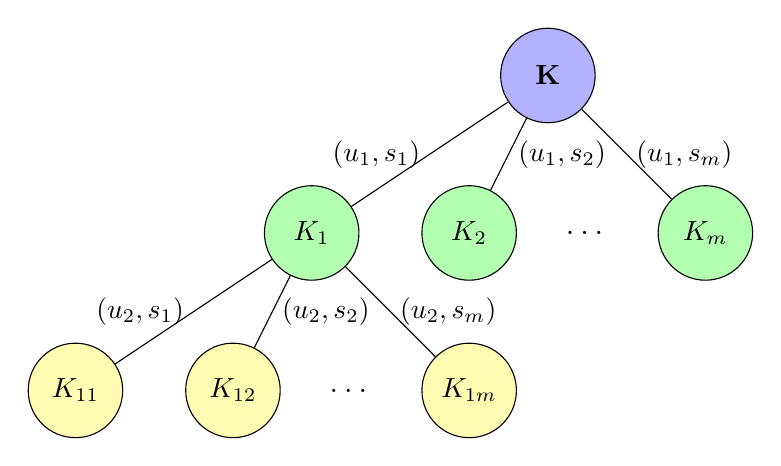
\begin{tikzpicture}
    \node[draw, circle, fill=blue!30, minimum size=12mm] (1) at (0,0) {\textbf{K}};
    
    \node[draw, circle, fill=green!30, minimum size=12mm] (2) at (-3,-2) {$K_1$};
    \draw (1) -- (2) node[pos=0.5, left] {$(u_1,s_1)$};
    \node[draw, circle, fill=green!30, minimum size=12mm] (3) at (-1,-2) {$K_2$};
    \draw (1) -- (3) node[pos=0.5, right] {$(u_1,s_2)$};
    \node[draw, circle, fill=green!30, minimum size=12mm] (5) at (2,-2) {$K_m$};
    \draw (1) -- (5) node[pos=0.5, right] {$(u_1,s_m)$};
    \node (4) at (0.5,-2) {\large \dots};


    \node[draw, circle, fill=yellow!30, minimum size=12mm] (6) at (-6,-4) {$K_{11}$};
    \draw (2) -- (6) node[pos=0.5, left] {$(u_2,s_1)$};
    \node[draw, circle, fill=yellow!30, minimum size=12mm] (7) at (-4,-4) {$K_{12}$};
    \draw (2) -- (7) node[pos=0.5, right] {$(u_2,s_2)$};
    \node (8) at (-2.5,-4) {\large \dots};
    \node[draw, circle, fill=yellow!30, minimum size=12mm] (9) at (-1,-4) {$K_{1m}$};
    \draw (2) -- (9) node[pos=0.5, right] {$(u_2,s_m)$};
    
    \end{tikzpicture}
    \caption{Strom o dvou tazích}
    \label{figcandidatetree}
    \end{figure}

\begin{figure}[h!]
    \centering
    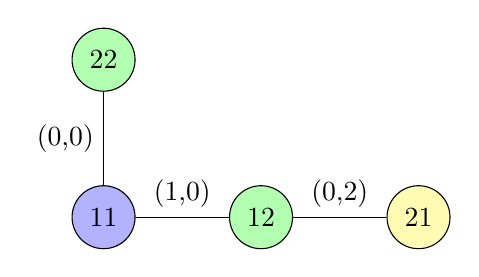
\begin{tikzpicture}
    \node[draw, circle, fill=blue!30, minimum size=8mm] (1) at (0,0) {11};
    \node[draw, circle, fill=green!30, minimum size=8mm] (2) at (0,2) {22};
    \draw (1) -- (2) node[pos=0.5, left] {(0,0)};
    \node[draw, circle, fill=green!30, minimum size=8mm] (3) at (2,0) {12};
    \draw (1) -- (3) node[pos=0.5, above] {(1,0)};
    \node[draw, circle, fill=yellow!30, minimum size=8mm] (4) at (4,0) {21};
    \draw (3) -- (4) node[pos=0.5, above] {(0,2)};
    \end{tikzpicture}
    \caption{Zahrané tahy podle ohodnocení}
    \label{fig23start12}
\end{figure}
